\documentclass[11pt]{article}
\usepackage{geometry}                % See geometry.pdf to learn the layout options. There are lots.
\geometry{letterpaper}                   % ... or a4paper or a5paper or ... 
%\geometry{landscape}                % Activate for for rotated page geometry
%\usepackage[parfill]{parskip}    % Activate to begin paragraphs with an empty line rather than an indent
\usepackage{graphicx}
\usepackage{amssymb}
\usepackage{epstopdf}
\usepackage{fixltx2e}			%provides \textsubscript
\DeclareGraphicsRule{.tif}{png}{.png}{`convert #1 `dirname #1`/`basename #1 .tif`.png}


%%
%% TIKZ for drawing DAGs (not sure how much of the below is necessary)
%%

\usepackage{tikz}
\usepackage{tkz-graph}
\usetikzlibrary{shapes,arrows}

\newcommand{\entrynode}[1]{
  \SetVertexNormal[Shape      = circle,
                   FillColor  = black,
                   LineWidth  = 0pt,
                   MinSize    = 0pt]
  \Vertex[L={\tiny\,}]{#1}
  \SetVertexNormal[Shape      = circle,
                   FillColor  = white,
                   LineWidth  = 2pt]
}

\SetUpEdge[lw         = 1.5pt,
           color      = black,
           labelcolor = white,
           labeltext  = red,
           labelstyle = {sloped,draw,text=blue}]

\tikzset{node distance = 2cm}




\title{Anonymity in XIA: Developer Tools and User Control}
\author{Nicolas Feltman and David Naylor}
\date{}                                           


\begin{document}
\maketitle
\section{Introduction}
The desire for anonymous communication in the Internet has made it a much-discussed issue in both technical and non-technical circles. Several standard approaches to anonymity have emerged, normally involving some number of explicitly identified proxies  due to the dumb nature of current routers. Although none of these methods are perfect, they generally meet most users' needs. Little work has been done, however, exploring ways to make these methods easily utilized by application developers and easily understood by end users.

Our goal is three-fold. First, we consider existing methods for achieving anonymous communication in the context of the eXpressive Internet Architecture (XIA). As we discuss below, novel features of XIA in many cases allow these existing techniques to be implemented more elegantly. Second, we introduce an anonymous socket API extension, which provides application developers a dead-easy way to use anonymous communication over XIA. Finally, we consider application users. Using the anonymous socket API, we will create a preference pane providing OS level control over the extended API functionality. Anonymization settings will be controllable by the user through an intuitive, easily understood GUI.

\subsection{XIA}
Some features of XIA have implications when it comes to anonymity. We briefly describe the key ideas here and elaborate on their impact on anonymous communication later.
\subsubsection{Principal-Based Communication}
In contrast with today's host-based Internet, XIA provides a framework for communication among \emph{principals}. The idea of principal-based communication is that users should be able to address packets directly to their primary \emph{intent}. For example, a user searching for books on Amazon wishes to communicate with \texttt{www.amazon.com}; he doesn't care which particular Amazon server responds to his request.

In this example, \texttt{www.amazon.com} can be viewed as a \emph{service} principal. In the case where communication with a particular machine truly is the intent, traditional host-based communication can still be achieved via the \emph{host} principal. Other principals include static \emph{content} (e.g. images) and \emph{autonomous domains} (similar to today's autonomous systems).

\subsubsection{DAG-Based Addressing}
Addresses in XIA are represented as DAGs (directed acyclic graphs). Using DAGs allows senders to give the network very detailed instructions about how a packet should be routed. DAGs also allow senders to provide {\em fallback} routes to be used in case the network cannot find the sender's primary intent or does not understand a new principal type. For example, in the scenario above, the user's browser might include the address of a particular Amazon server as a backup in case a packet reaches a router that doesn't know how to find the service \texttt{www.amazon.com} directly.

\begin{figure}
\centering
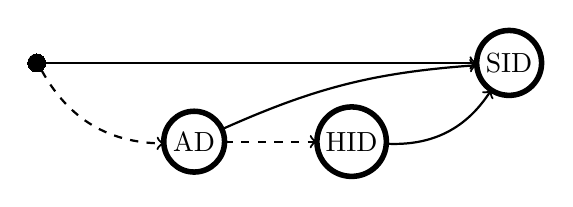
\begin{tikzpicture}
  \entrynode{A}
  \Vertex[x=6,y=0,L=SID]{B}
  \Vertex[x=2,y=-1,L=AD]{C}
  \Vertex[x=4,y=-1,L=HID]{D}
  \tikzstyle{EdgeStyle}=[->]
  \Edge(A)(B)
  \tikzstyle{EdgeStyle}=[dashed, bend right, ->]
  \Edge(A)(C)
  \tikzstyle{EdgeStyle}=[bend left=10, ->]
  \Edge(C)(B)
  \tikzstyle{EdgeStyle}=[dashed, ->]
  \Edge(C)(D)
  \tikzstyle{EdgeStyle}=[bend right, ->]
  \Edge(D)(B)
\end{tikzpicture}
\caption{A typical DAG with two fallbacks. Note that higher edges have higher priority; SID is the primary intent, so the network attempts to route it first. If a router does not know the location of SID, or does not understand services, it uses the first fallback and instead routes the packet to SID's AD. Once in the AD, if a router cannot find SID, the packet is routed to HID, the second fallback, before finally being delivered to the service.}
\label{fig:proxy-service}
\end{figure}


\subsubsection{Intrinsic Security}
All addresses (or, better put, identifiers) in XIA are \emph{intrinsically secure}; exactly what this means varies among principals. For example, a content identifier (CID) is the cryptographic hash of the content itself, enabling anyone receiving the content to verify its integrity. Hosts and services are required to have a public/private key pair; therefore their corresponding identifiers (HIDs and SIDs) are simply the hashes of public keys. A host can sign any communication it generates with its private key and anyone can publicly verify the signature using the host's ID.


\section{Levels of Anonymity}
We adopt terminology proposed by Pfitzmann and K\"{o}hntopp to precisely describe varying degrees of anonymity:
\begin{description}
\item[Anonymity] The state of not being identifiable within a set of subjects, the {\em anonymity set}.
\item[Unlinkability] Two or more items (e.g., subjects, messages, events, actions, etc.) are no more and no less related than they are related to any other item.
\item[Sender Anonymity] A particular message is not linkable to any sender and no message is linkable to a particular sender.
\item[Recipient Anonymity] A particular message cannot be linked to any recipient and no message is linkable to a particular recipient.
\item[Unobservability] The state of messages being indistinguishable from no messages at all.
\end{description}

\section{Approach: Proxies}
The first approach we will discuss for providing anonymity is the use of {\em proxies}.  The client hides its identify by routing all of its communications with a service provider through an auxiliary party called a proxy.  Since the service provider only ever interacts with the proxy and never with the client directly, it does not need to know the identity (in XIA, the host ID) of the requester.

In this section we will describe one possible way to implement a proxy protocol as an in-network service in XIA.  

\subsection{Proxy Addresses}

One key feature of our proxy protocol design is including the proxy's address with the address of the final service provider in a single DAG.  This means that from the point of view of a client application developer, the use of a proxy can be expressed entirely within the end service's address DAG. Although we considered introducing a new principal type for proxy services, we found that they could be expressed sufficiently with the standard service principal type.  The DAG in Figure~\ref{fig:proxy-service} represents communication with the end service SID\textsubscript{E} via the proxy SID\textsubscript{P}, with fallback paths for both.  We do not cover in this document how the proxy's DAG is obtained.

\begin{figure}
\centering
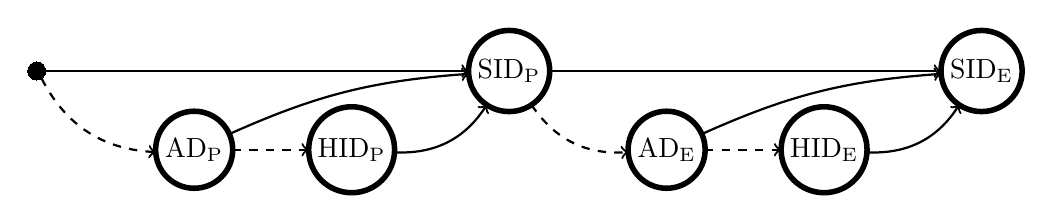
\begin{tikzpicture}
  \entrynode{A}
  \Vertex[x=6,y=0,L=SID\textsubscript{P}]{B}
  \Vertex[x=2,y=-1,L=AD\textsubscript{P}]{C}
  \Vertex[x=4,y=-1,L=HID\textsubscript{P}]{D}
  \Vertex[x=12,y=0,L=SID\textsubscript{E}]{E}
  \Vertex[x=8,y=-1,L=AD\textsubscript{E}]{F}
  \Vertex[x=10,y=-1,L=HID\textsubscript{E}]{G}
  \tikzstyle{EdgeStyle}=[->]
  \Edge(A)(B)
  \tikzstyle{EdgeStyle}=[dashed, bend right, ->]
  \Edge(A)(C)
  \tikzstyle{EdgeStyle}=[bend left=10, ->]
  \Edge(C)(B)
  \tikzstyle{EdgeStyle}=[dashed, ->]
  \Edge(C)(D)
  \tikzstyle{EdgeStyle}=[bend right, ->]
  \Edge(D)(B)
  \tikzstyle{EdgeStyle}=[->]
  \Edge(B)(E)
  \tikzstyle{EdgeStyle}=[dashed, bend right, ->]
  \Edge(B)(F)
  \tikzstyle{EdgeStyle}=[bend left=10, ->]
  \Edge(F)(E)
  \tikzstyle{EdgeStyle}=[dashed, ->]
  \Edge(F)(G)
  \tikzstyle{EdgeStyle}=[bend right, ->]
  \Edge(G)(E)
\end{tikzpicture}
\caption{A host can use an in-network proxy service with a DAG like this one.}
\label{fig:proxy-service}
\end{figure}

\subsection{Protocol}

This version of the protocol assumes that the client application does not need to communicate any connection parameters with proxy.  The client begins by obtaining DAGs for the proxy and for the end service.  Let the proxy service have the public address SID\textsubscript{P} and the end service have the address SID\textsubscript{E}. Let the client application be running on a host HID\textsubscript{C} with an ephemeral service identifier SID\textsubscript{A} (for demultiplexing).  It sends the initial packet with the following destination and source addresses (fallback paths omitted):

\begin{center}
    \begin{tabular}{ | l | l |} \hline
    	Dst & Src \\ 
	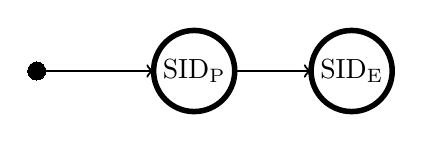
\begin{tikzpicture}
	\entrynode{A}
	\Vertex[x=2,y=0,L=SID\textsubscript{P}]{P}
	\Vertex[x=4,y=0,L=SID\textsubscript{E}]{E}
	\tikzstyle{EdgeStyle}=[->]
	\Edge(A)(P)
	\tikzstyle{EdgeStyle}=[->]
	\Edge(P)(E)
	\end{tikzpicture} &
	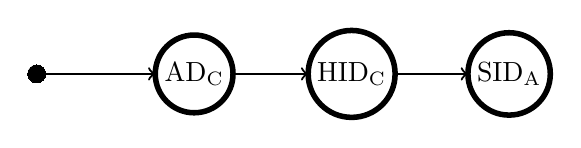
\begin{tikzpicture}
	\entrynode{B}
	\Vertex[x=2,y=0,L=AD\textsubscript{C}]{A}
	\Vertex[x=4,y=0,L=HID\textsubscript{C}]{H}
	\Vertex[x=6,y=0,L=SID\textsubscript{A}]{S}
	\tikzstyle{EdgeStyle}=[->]
	\Edge(B)(A)
	\tikzstyle{EdgeStyle}=[->]
	\Edge(A)(H)
	\tikzstyle{EdgeStyle}=[->]
	\Edge(H)(S)
	\end{tikzpicture}
    \\ \hline
    \end{tabular}
\end{center}

Upon receiving this initial packet, the proxy service routes it to a particular machine, henceforth HID\textsubscript{P}, to handle this connection. Since this is the first packet from AD\textsubscript{C}:HID\textsubscript{C}:SID\textsubscript{A}, the proxy creates a new ephemeral service ID, SID\textsubscript{T} and adds this pair to a local table. (Responses from the end service, SID\textsubscript{E}, are sent to the proxy at SID\textsubscript{T}, which looks up the client address corresponding to SID\textsubscript{T} in it's table and forwards the response to the appropriate address.) The machine then forwards the initial packet with the following destination and source addresses:

\begin{center}
    \begin{tabular}{ | l | l |} \hline
    	Dst & Src \\ 
	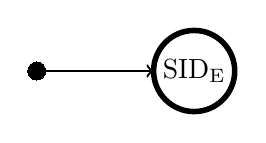
\begin{tikzpicture}
	\entrynode{A}
	\Vertex[x=2,y=0,L=SID\textsubscript{E}]{E}
	\tikzstyle{EdgeStyle}=[->]
	\Edge(A)(E)
	\end{tikzpicture} &
	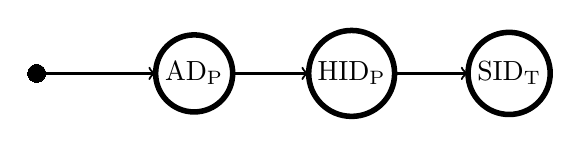
\begin{tikzpicture}
	\entrynode{B}
	\Vertex[x=2,y=0,L=AD\textsubscript{P}]{A}
	\Vertex[x=4,y=0,L=HID\textsubscript{P}]{H}
	\Vertex[x=6,y=0,L=SID\textsubscript{T}]{S}
	\tikzstyle{EdgeStyle}=[->]
	\Edge(B)(A)
	\tikzstyle{EdgeStyle}=[->]
	\Edge(A)(H)
	\tikzstyle{EdgeStyle}=[->]
	\Edge(H)(S)
	\end{tikzpicture}
    \\ \hline
    \end{tabular}
\end{center}

The end service is not aware that it is being communicated with via a proxy. It chooses a machine, HID\textsubscript{E}, to handle this connection, and responds with the following source and destination addresses:

\begin{center}
    \begin{tabular}{ | l | l |} \hline
    	Dst & Src \\
	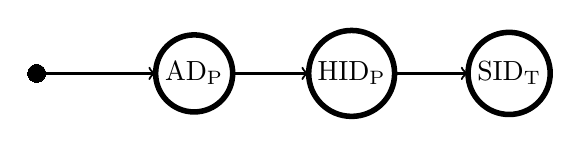
\begin{tikzpicture}
	\entrynode{B}
	\Vertex[x=2,y=0,L=AD\textsubscript{P}]{A}
	\Vertex[x=4,y=0,L=HID\textsubscript{P}]{H}
	\Vertex[x=6,y=0,L=SID\textsubscript{T}]{S}
	\tikzstyle{EdgeStyle}=[->]
	\Edge(B)(A)
	\tikzstyle{EdgeStyle}=[->]
	\Edge(A)(H)
	\tikzstyle{EdgeStyle}=[->]
	\Edge(H)(S)
	\end{tikzpicture} &
	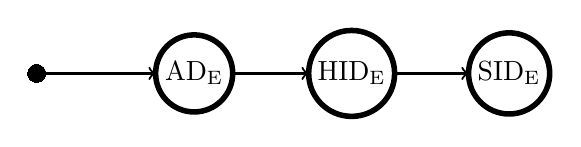
\begin{tikzpicture}
	\entrynode{B}
	\Vertex[x=2,y=0,L=AD\textsubscript{E}]{A}
	\Vertex[x=4,y=0,L=HID\textsubscript{E}]{H}
	\Vertex[x=6,y=0,L=SID\textsubscript{E}]{S}
	\tikzstyle{EdgeStyle}=[->]
	\Edge(B)(A)
	\tikzstyle{EdgeStyle}=[->]
	\Edge(A)(H)
	\tikzstyle{EdgeStyle}=[->]
	\Edge(H)(S)
	\end{tikzpicture}
    \\ \hline
    \end{tabular}
\end{center}

The proxy, in the interest of keeping minimal state, does not remember this bound source address but instead simply sends it back to the client who is responsible for including HID\textsubscript{E} in future packets.

\begin{center}
    \begin{tabular}{ | l |} \hline
    	Dst \\ 
	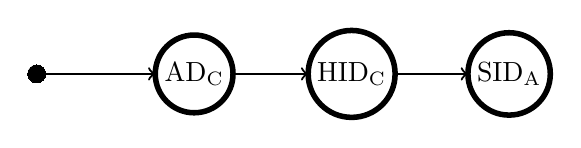
\begin{tikzpicture}
	\entrynode{B}
	\Vertex[x=2,y=0,L=AD\textsubscript{C}]{A}
	\Vertex[x=4,y=0,L=HID\textsubscript{C}]{H}
	\Vertex[x=6,y=0,L=SID\textsubscript{A}]{S}
	\tikzstyle{EdgeStyle}=[->]
	\Edge(B)(A)
	\tikzstyle{EdgeStyle}=[->]
	\Edge(A)(H)
	\tikzstyle{EdgeStyle}=[->]
	\Edge(H)(S)
	\end{tikzpicture} \\ \hline
	Src \\ 
	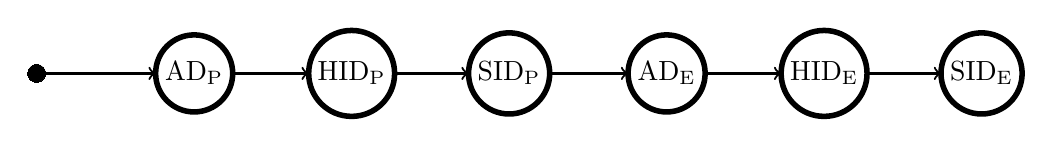
\begin{tikzpicture}
	\entrynode{B}
	\Vertex[x=2,y=0,L=AD\textsubscript{P}]{A}
	\Vertex[x=4,y=0,L=HID\textsubscript{P}]{H}
	\Vertex[x=6,y=0,L=SID\textsubscript{P}]{S}
	\Vertex[x=8,y=0,L=AD\textsubscript{E}]{A2}
	\Vertex[x=10,y=0,L=HID\textsubscript{E}]{H2}
	\Vertex[x=12,y=0,L=SID\textsubscript{E}]{S2}
	\tikzstyle{EdgeStyle}=[->]
	\Edge(B)(A)
	\tikzstyle{EdgeStyle}=[->]
	\Edge(A)(H)
	\tikzstyle{EdgeStyle}=[->]
	\Edge(H)(S)
	\tikzstyle{EdgeStyle}=[->]
	\Edge(S)(A2)
	\tikzstyle{EdgeStyle}=[->]
	\Edge(A2)(H2)
	\tikzstyle{EdgeStyle}=[->]
	\Edge(H2)(S2)
	\end{tikzpicture}
    \\ \hline
    \end{tabular}
\end{center}

The client receives the bound source DAG, sending all future communications to it. Thus, the client continues communicating with the host via the proxy, which swaps references to AD\textsubscript{C}:HID\textsubscript{C}:SID\textsubscript{A} with AD\textsubscript{P}:HID\textsubscript{P}:SID\textsubscript{T}, and the end service thinks it is maintaining a persistent connection with AD\textsubscript{P}:HID\textsubscript{P}:SID\textsubscript{T}.  

\section{Approach: Temporary Service IDs}

Our second method for anonymization involves explicit cooperation of the client's AD.  In this method, the client requests a temporary service ID, or {\em pseudonym}, from the AD through a special mechanism.  It then uses this pseudonym (bound within the AD) as its return address.  This level of anonymity is accepable for some applications.  

\subsection{Protocol}

The client, running on host HID\textsubscript{C}, starts by requesting a psuedonym from its administrative domain, which has the address AD\textsubscript{C}.  The AD, which must explicitly support this operation, then generates a temporary service identifier, SID\textsubscript{N}, and propagates forwarding information SID\textsubscript{N}$\rightarrow$HID\textsubscript{C} to its routers. Note that it is critical that AD\textsubscript{C} not advertise this information to other ADs; only it knows the association between SID\textsubscript{N} and HID\textsubscript{C} From here, the client simply uses the following DAG as the source address in its packets, excluding the usual HID\textsubscript{C} node:

\begin{center}
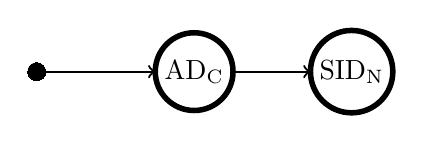
\begin{tikzpicture}
	\entrynode{B}
	\Vertex[x=2,y=0,L=AD\textsubscript{C}]{A}
	\Vertex[x=4,y=0,L=SID\textsubscript{N}]{H}
	\tikzstyle{EdgeStyle}=[->]
	\Edge(B)(A)
	\tikzstyle{EdgeStyle}=[->]
	\Edge(A)(H)
\end{tikzpicture}
\end{center}

\section{An API for Developers}
As we have discussed above, XIA allows for simple, if not elegant, ways to employ techniques for anonymization. For instance, we explored how an application can achieve fine-grain control over the use of a proxy service through DAG manipulation. We also proposed the use of temporary SIDs as pseudonyms.

Both of these strategies incorporate anonymity by leveraging core features of XIA. Thus, it is both possible and useful to provide a standard set of tools implementing these techniques to application developers --- it would be silly for each developer to implement his/her own functions for adding a proxy service to all outgoing DAGs, for example.

We will implement these tools in the form of an extension to the XSocket API. (The XSocket API, as the name suggests, allows developers to communicate with sockets over XIA, much like network applications today use TCP or UDP sockets.) These new functions allow developers to specify how they want to achieve anonymity (i.e., by routing traffic through a proxy of their choice) just once, after which they can send packets using the specified service with no extra effort, using the standard \texttt{XSend()} and \texttt{XRecv()} calls. In \S~\ref{sec:api-interface} we present the interface of our extension to the XSocket API. (As our implementation will involve repeated manipulation of DAGs, we also propose new standard DAG manipulation functions. We expect this list to grow as we implement the new API functions.)

\subsection{DAG Library Extension}

\begin{center}
	\begin{tabular}{l p{7cm}}
	\textbf{Function} 	&	\textbf{Description}\\
	\hline
	\texttt{AppendDag(dag1, dag2)} & Appends \texttt{dag2} to the end of \texttt{dag1}.  This is used to create a proxy-routed address. \\ \hline
	\end{tabular}
\end{center}

\subsection{XSocket API Extension}
\label{sec:api-interface}

\begin{center}
	\begin{tabular}{l p{7cm}}
	\textbf{Function} 	&	\textbf{Description}\\
	\hline
	\texttt{XEnableAnonymizer()} & Instructs the socket layer to route all traffic through an anonymization service. If none is specified, a default is used.\\
	\texttt{XDisableAnonymizer()} & Instructs the socket layer not to use an anonymization service.\\
	\texttt{XSetAnonymizer(dag)} & Sets the DAG of an anonymization service.\\
	\texttt{XEnableTemporarySID()} & Instructs the socket layer to use a temporary SID as a source address.\\
	\texttt{XSetTemporarySIDDuration(duration)} & Sets the duration of temporary SIDs to \texttt{duration} seconds. When a temporary SID expires, a new one is generated.\\
	\hline
	\end{tabular}
\end{center}

\section{System-Wide User Controls}
By introducing an anonymization preference pane, we allow users to ensure that all outbound traffic from their system is anonymized according to the specified settings (Figure~\ref{fig:system_anon_settings}).

\begin{figure}
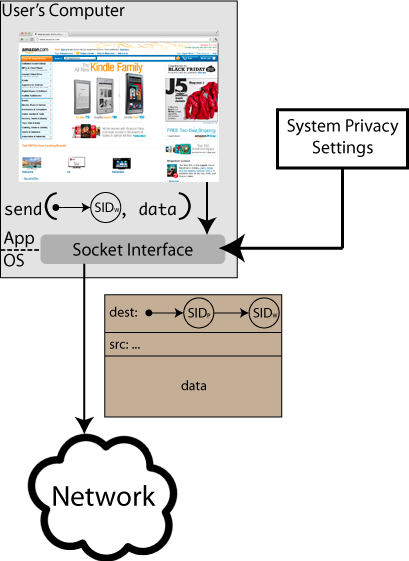
\includegraphics{images/system_anon_settings.png}
\caption{System-wide controls bypass applications entirely, allowing users to ensure all traffic is sent as per their anonymization settings.}
\label{fig:system_anon_settings}
\end{figure}



\end{document}  